% This file was created by matlab2tikz.
%
%The latest updates can be retrieved from
%  http://www.mathworks.com/matlabcentral/fileexchange/22022-matlab2tikz-matlab2tikz
%where you can also make suggestions and rate matlab2tikz.
%
\definecolor{mycolor1}{rgb}{0.00000,0.44700,0.74100}%
\definecolor{mycolor2}{rgb}{0.92900,0.69400,0.12500}%
\definecolor{mycolor3}{rgb}{0.46600,0.67400,0.18800}%
\definecolor{mycolor4}{rgb}{0.63500,0.07800,0.18400}%
\definecolor{mycolor5}{rgb}{0.85000,0.32500,0.09800}%
%
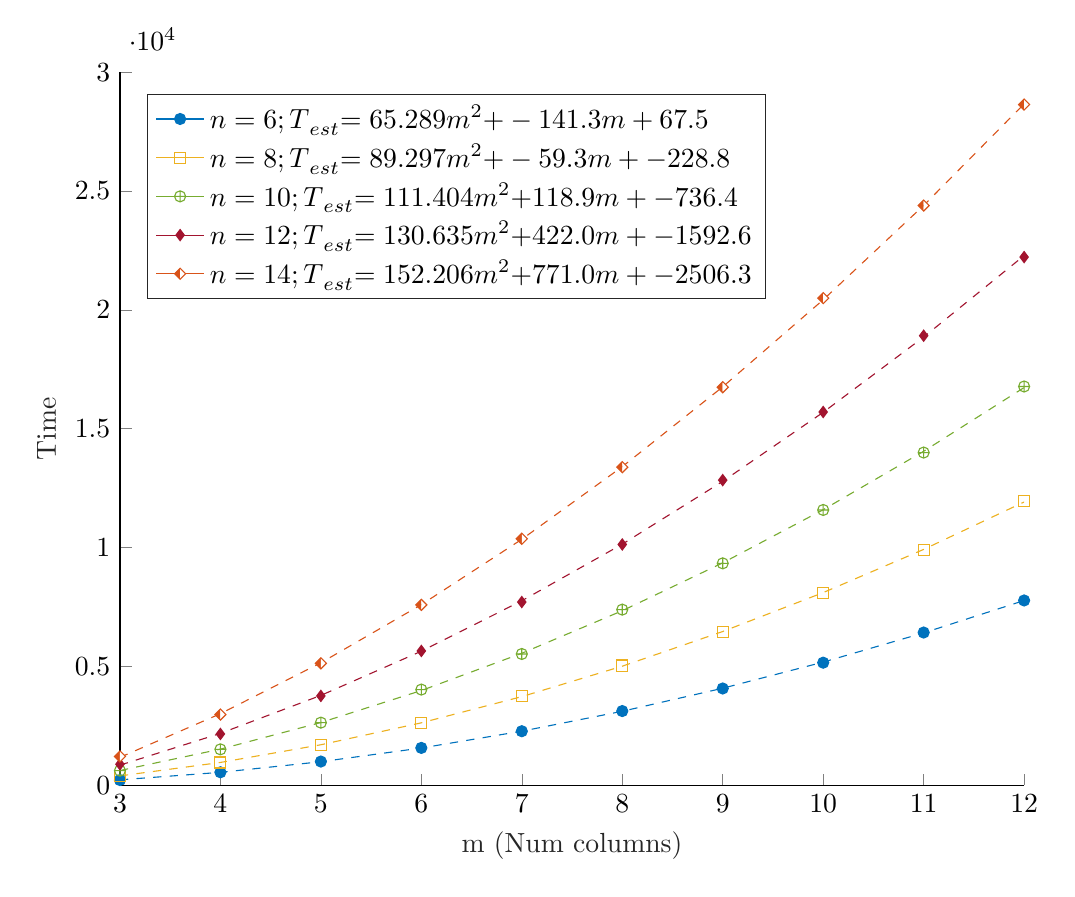
\begin{tikzpicture}

\begin{axis}[%
width=4.521in,
height=3.566in,
at={(0.758in,0.481in)},
scale only axis,
xmin=3,
xmax=12,
xlabel style={font=\color{white!15!black}},
xlabel={m (Num columns)},
ymin=0,
ymax=30000,
ylabel style={font=\color{white!15!black}},
ylabel={Time},
axis background/.style={fill=white},
title style={font=\bfseries},
% title={$\text{Average ticks until solution as a function of m. On n }\times\text{ m grid. (k = 1)}$},
axis x line*=bottom,
axis y line*=left,
legend style={at={(0.03,0.97)}, anchor=north west, legend cell align=left, align=left, draw=white!15!black}
]
\addplot [color=mycolor1, draw=none, mark=*, mark options={solid, mycolor1}]
  table[row sep=crcr]{%
3	222.472\\
4	549.578\\
5	1001.042\\
6	1575.098\\
7	2276.66\\
8	3124.486\\
9	4074.182\\
10	5159.664\\
11	6427.76\\
12	7776.634\\
};
\addlegendentry{$\text{n =  6; T}_{\text{est}}\text{ =  65.289m}^\text{2}\text{ + -141.3m +    67.5}$}

\addplot [color=mycolor1, dashed, forget plot]
  table[row sep=crcr]{%
3	231.140781818178\\
4	546.849933333331\\
5	993.136221212121\\
6	1569.99964545455\\
7	2277.44020606061\\
8	3115.4579030303\\
9	4084.05273636364\\
10	5183.22470606061\\
11	6412.97381212121\\
12	7773.30005454545\\
};
\addplot [color=mycolor2, draw=none, mark=square, mark options={solid, mycolor2}]
  table[row sep=crcr]{%
3	394.614\\
4	960.756\\
5	1702.446\\
6	2631.208\\
7	3744.352\\
8	5038.374\\
9	6450.922\\
10	8104.354\\
11	9883.782\\
12	11950.274\\
};
\addlegendentry{$\text{n =  8; T}_{\text{est}}\text{ =  89.297m}^\text{2}\text{ +  -59.3m +  -228.8}$}

\addplot [color=mycolor2, dashed, forget plot]
  table[row sep=crcr]{%
3	396.990672727258\\
4	962.768103030298\\
5	1707.13879090909\\
6	2630.10273636364\\
7	3731.65993939395\\
8	5011.81040000001\\
9	6470.55411818182\\
10	8107.8910939394\\
11	9923.82132727272\\
12	11918.3448181818\\
};
\addplot [color=mycolor3, draw=none, mark=oplus, mark options={solid, mycolor3}]
  table[row sep=crcr]{%
3	618.156\\
4	1513.952\\
5	2637.64\\
6	4027.648\\
7	5525.28\\
8	7391.572\\
9	9337.908\\
10	11583.686\\
11	13998.248\\
12	16777.122\\
};
\addlegendentry{$\text{n = 10; T}_{\text{est}}\text{ = 111.404m}^\text{2}\text{ +  118.9m +  -736.4}$}

\addplot [color=mycolor3, dashed, forget plot]
  table[row sep=crcr]{%
3	623.022345454534\\
4	1521.77833333333\\
5	2643.3423969697\\
6	3987.71453636364\\
7	5554.89475151516\\
8	7344.88304242425\\
9	9357.67940909091\\
10	11593.2838515152\\
11	14051.696369697\\
12	16732.9169636364\\
};
\addplot [color=mycolor4, draw=none, mark=diamond*, mark options={solid, mycolor4}]
  table[row sep=crcr]{%
3	887.67\\
4	2160.546\\
5	3762.974\\
6	5653.65\\
7	7710.138\\
8	10132.224\\
9	12838.396\\
10	15703.31\\
11	18914.808\\
12	22220.482\\
};
\addlegendentry{$\text{n = 12; T}_{\text{est}}\text{ = 130.635m}^\text{2}\text{ +  422.0m + -1592.6}$}

\addplot [color=mycolor4, dashed, forget plot]
  table[row sep=crcr]{%
3	849.140818181802\\
4	2185.5917030303\\
5	3783.31342121212\\
6	5642.30597272728\\
7	7762.56935757577\\
8	10144.1035757576\\
9	12786.9086272727\\
10	15690.9845121212\\
11	18856.331230303\\
12	22282.9487818182\\
};
\addplot [color=mycolor5, draw=none, mark=halfsquare left*, mark options={solid, mycolor5}]
  table[row sep=crcr]{%
3	1215.818\\
4	2978.586\\
5	5131.972\\
6	7592.148\\
7	10372.798\\
8	13382.324\\
9	16746.834\\
10	20494.166\\
11	24387.434\\
12	28636.5\\
};
\addlegendentry{$\text{n = 14; T}_{\text{est}}\text{ = 152.206m}^\text{2}\text{ +  771.0m + -2506.3}$}

\addplot [color=mycolor5, dashed, forget plot]
  table[row sep=crcr]{%
3	1176.71250909097\\
4	3013.20189090911\\
5	5154.1032121212\\
6	7599.41647272724\\
7	10349.1416727272\\
8	13403.2788121212\\
9	16761.8278909091\\
10	20424.7889090909\\
11	24392.1618666667\\
12	28663.9467636364\\
};
\end{axis}
\end{tikzpicture}%
